% THIS IS GDANSK UNIVERSITY OF TECHNLOGOGY (PG) PRESENTATION TEMPLATE
% Creator: Jan Cychnerski <jan.cychnerski@eti.pg.edu.pl>
% Copyleft 2019

% traditional screen
%\documentclass{beamer}

% wide screen
\documentclass[aspectratio=169]{beamer}


%%% YOUR PACKAGES HERE %%%
\usepackage{comment}
\usepackage{hyperref}
\usepackage{graphicx}
\usepackage{caption}


% polish language
\usepackage[polish]{babel}
\usepackage{polski}


%%% IMPORT PG PRESENTATION STYLE %%%
% THIS IS GDANSK UNIVERSITY OF TECHNLOGOGY (PG) PRESENTATION TEMPLATE
% Creator: Jan Cychnerski <jan.cychnerski@eti.pg.edu.pl>
% Copyleft 2019


% PG THEME OPTIONS

\usetheme{Boadilla}
\usecolortheme{default}
\usefonttheme{professionalfonts}

% colors

\definecolor{PGBlue}{RGB}{0,56,101}
\definecolor{PGRed}{RGB}{193,10,39}
\definecolor{PGSilver}{RGB}{200,200,200}
\definecolor{PGBlack}{RGB}{0,0,0}

% PGBlue
\setbeamercolor{frametitle}{fg=PGBlue}
\setbeamercolor{normal text}{fg=PGBlue}
\setbeamercolor{structure}{fg=PGBlue}
\setbeamercolor{item}{fg=PGBlue}

% PGRed
\setbeamercolor{alerted text}{fg=PGRed}
\setbeamercolor{item projected}{fg=PGRed}

% white
\setbeamercolor{title}{fg=white}
\setbeamercolor{titlelike}{fg=white}
\setbeamercolor{subtitle}{fg=white}

% enumerate and itemize styles

\setbeamertemplate{itemize item}{\bfseries\color{PGRed}\raise1pt\hbox{\donotcoloroutermaths$\bullet$}}
\setbeamertemplate{itemize subitem}{\color{PGRed}\raise0.5pt\hbox{--}}
\setbeamertemplate{itemize subsubitem}{\color{PGRed}\tiny\raise1.5pt\hbox{\donotcoloroutermaths$\bullet$}}

\setbeamertemplate{enumerate item}{\bfseries\color{PGRed}\insertenumlabel.}
\setbeamertemplate{enumerate subitem}{\color{PGRed}\insertsubenumlabel.}
\setbeamertemplate{enumerate subsubitem}{\color{PGRed}\insertsubsubenumlabel.}
\setbeamertemplate{enumerate mini template}{\insertenumlabel}


% disable navigation

\beamertemplatenavigationsymbolsempty

% additional commands

\newcommand*{\vcenteredhbox}[1]{\begingroup
\setbox0=\hbox{#1}\parbox{\wd0}{\box0}\endgroup}

\graphicspath{{pgbeamer/}}


\usepackage{iflang}
\IfLanguageName{polish}{
\newcommand{\pglogobig}{pg-logo-big-pl}
\newcommand{\pglogosmall}{pg-logo-small-pl}
}{
\newcommand{\pglogobig}{pg-logo-big-en}
\newcommand{\pglogosmall}{pg-logo-small-en}
}


% FRAME TITLE LOGO
\addtobeamertemplate{frametitle}{\vcenteredhbox{\includegraphics[height=8mm]{\pglogosmall}}\bfseries}{}


\newcommand{\pgtitleframe}{{
% PG TITLE PAGE

\setbeamercolor{background canvas}{bg=PGBlue}
\setbeamercolor{title}{fg=white}
\setbeamercolor*{date}{fg=white}
\setbeamercolor*{author}{fg=white}

\setbeamertemplate{footline}{}

\begin{frame}[noframenumbering]
\centering
\vspace{1cm}
\includegraphics[height=3cm]{\pglogobig}
\vspace{5mm}
\maketitle
\end{frame}
}}

\newcommand{\pglastframe}{{
% PG LAST PAGE

\setbeamercolor{background canvas}{bg=PGBlue}
\setbeamercolor{title}{fg=white}
\setbeamercolor*{date}{fg=white}
\setbeamercolor*{author}{fg=white}

\setbeamertemplate{footline}{}

\begin{frame}[noframenumbering]
\centering
\vspace{1cm}
\includegraphics[height=5cm]{\pglogobig}
\end{frame}
}}



%%% YOUR OPTIONS HERE %%%

\title[PG Presentation]{Licencjonowanie w kryptografii}
\author{inż. Mikołaj Nowak \and inż. Jakub Grzybowski \and inż. Wojciech Baranowski}
\date{\today}

%%% DOCUMENT BEGINS HERE %%%

\begin{document}

%%% PG TITLE PAGE %%%
\pgtitleframe

%%% YOUR PRESENTATION HERE %%%

\setbeamercovered{invisible}
\author{M. Nowak \and J. Grzybowski \and W. Baranowski}

\begin{frame}{Czym jest stos TCP/IP?}
  \begin{columns}
    \begin{column}{0.55\textwidth}
      \begin{itemize}
        \item Zestaw protokołów komunikacyjnych używanych w sieciach komputerowych.
        \item Obejmuje cztery główne warstwy:
        \begin{itemize}
          \item Aplikacji
          \item Transportową
          \item Internetową
          \item Dostępu do sieci
        \end{itemize}
        \item Jest zaimplementowany jako część jądra systemu operacyjnego.
        \item Umożliwia komunikację w Internecie i sieciach lokalnych.
      \end{itemize}
    \end{column}
    \begin{column}{0.4\textwidth}
      \centering
      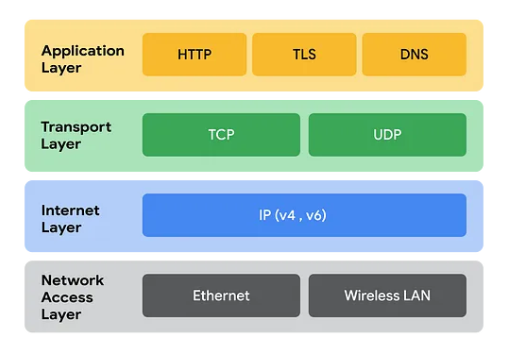
\includegraphics[width=\linewidth]{tcpip.png}
    \end{column}
  \end{columns}
\end{frame}

\begin{frame}{Rodzaje licencji oprogramowania}
  \begin{itemize}
    \item \textbf{Otwarte licencje (Open Source):}
    \begin{itemize}
      \item \textbf{GPL (GNU General Public License):} wymaga udostępnienia kodu źródłowego oraz wszelkich zmian – tzw. \textit{copyleft}.
      \item \textbf{BSD, MIT:} pozwalają na modyfikację i wykorzystanie komercyjne bez obowiązku udostępniania zmian.
    \end{itemize}
    \vspace{0.5em}
    \item \textbf{Zamknięte licencje (Proprietary):}
    \begin{itemize}
      \item Kod źródłowy nie jest publicznie dostępny.
      \item Brak możliwości legalnej modyfikacji i redystrybucji.
      \item Oprogramowanie objęte licencją końcowego użytkownika (\textit{EULA}).
    \end{itemize}
    \vspace{0.5em}
    \item Licencje wpływają na rozwój, bezpieczeństwo i elastyczność oprogramowania.
  \end{itemize}
\end{frame}

\begin{frame}{Znaczenie licencji dla stosu TCP/IP}
  \begin{itemize}
    \item Implementacja stosu TCP/IP jest zwykle częścią jądra systemu operacyjnego.
    \item Licencja jądra decyduje o:
    \begin{itemize}
      \item dostępie do kodu źródłowego stosu,
      \item możliwości modyfikacji i ponownego rozpowszechniania,
      \item integracji z innym oprogramowaniem (np. komercyjnym).
    \end{itemize}
    \vspace{0.5em}
    \item \textbf{Otwarte jądra} (np. Linux, BSD) pozwalają na:
    \begin{itemize}
      \item audyt bezpieczeństwa,
      \item eksperymenty naukowe i edukacyjne,
      \item tworzenie niestandardowych rozszerzeń.
    \end{itemize}
    \vspace{0.5em}
    \item \textbf{Zamknięte jądra} (np. Windows, iOS) ograniczają kontrolę nad działaniem sieci.
  \end{itemize}
\end{frame}

\begin{frame}{Linux}
  \begin{itemize}
    \item Jądro Linuxa jest licencjonowane na zasadach \textbf{GPLv2 (GNU General Public License)}.
    \item Stos TCP/IP jest jego integralną częścią – licencja obejmuje cały kod źródłowy.
    \item Użytkownicy mają pełen dostęp do kodu, mogą go:
    \begin{itemize}
      \item analizować,
      \item modyfikować,
      \item dystrybuować dalej (z zachowaniem GPL).
    \end{itemize}
    \item Bogate możliwości rozszerzania dzięki modułom takim jak:
    \begin{itemize}
      \item \texttt{netfilter}, \texttt{nftables} – filtrowanie pakietów,
      \item \texttt{eBPF} – dynamiczne programowanie zachowania stosu w jądrze.
    \end{itemize}
    \item Wykorzystywany w wielu środowiskach: od serwerów i komputerów po Androida i IoT.
  \end{itemize}
\end{frame}

\begin{frame}{macOS / iOS}
  \begin{itemize}
    \item Systemy Apple bazują na \textbf{Darwinie} – jądrze typu Unix, opartym częściowo na \textbf{FreeBSD}.
    \item Część komponentów (w tym fragmenty stosu TCP/IP) pochodzi z BSD i są dostępne na licencji \textbf{BSD}.
    \item Apple jednak wprowadza własne rozszerzenia i modyfikacje, które:
    \begin{itemize}
      \item nie są publicznie dostępne,
      \item objęte są licencjami zastrzeżonymi,
      \item mogą być zamknięte mimo otwartego „rdzenia”.
    \end{itemize}
    \item Oficjalna licencja źródłowego Darwina: \textbf{APSL (Apple Public Source License)} – niezgodna z GPL, uważana za problematyczną.
    \item Stos TCP/IP w macOS/iOS to więc:
    \begin{itemize}
      \item kombinacja komponentów BSD,
      \item zamkniętych rozszerzeń Apple,
      \item fragmentów o niejednoznacznym statusie licencyjnym.
    \end{itemize}
  \end{itemize}
\end{frame}

\begin{frame}{Windows}
  \begin{itemize}
    \item Systemy Windows korzystają z własnościowego stosu TCP/IP – zamkniętego i niedostępnego publicznie.
    \item Stos został zaimplementowany samodzielnie przez Microsoft – początkowo w Windows NT, dziś obecny we wszystkich wersjach.
    \item Brak dostępu do kodu źródłowego oznacza:
    \begin{itemize}
      \item brak możliwości modyfikacji lub audytu,
      \item pełną zależność od aktualizacji Microsoftu,
      \item niemożność dostosowania do nietypowych zastosowań.
    \end{itemize}
    \item Licencjonowanie odbywa się wraz z systemem – użytkownik akceptuje \textit{EULA}, bez wpływu na wewnętrzne komponenty.
    \item Dla programistów dostępne są tylko wysokopoziomowe API (np. WinSock), ale nie kod źródłowy implementacji.
  \end{itemize}
\end{frame}

\begin{frame}{BSD (FreeBSD / OpenBSD / NetBSD)}
  \begin{itemize}
    \item Rodzina systemów BSD korzysta z licencji \textbf{BSD} – bardziej liberalnej niż GPL.
    \item Licencja pozwala na:
    \begin{itemize}
      \item modyfikację i dowolne wykorzystanie kodu,
      \item zamknięcie kodu w produktach komercyjnych bez obowiązku publikacji zmian.
    \end{itemize}
    \item \textbf{FreeBSD} – popularny w serwerach i systemach NAS (np. TrueNAS).
    \item \textbf{OpenBSD} – znany z nacisku na bezpieczeństwo i audyt kodu.
    \item \textbf{NetBSD} – ekstremalnie przenośny, działa na setkach architektur.
    \item Kod stosu TCP/IP z BSD jest wykorzystywany m.in. w:
    \begin{itemize}
      \item MacOS i iOS (częściowo)
      \item Juniper JunOS,
      \item Sony PlayStation.
    \end{itemize}
  \end{itemize}
\end{frame}

\begin{frame}{RouterOS / VxWorks / Cisco IOS}
  \begin{itemize}
    \item Systemy te są ściśle powiązane ze sprzętem i mają wbudowany, zamknięty stos TCP/IP.
    \item \textbf{RouterOS (MikroTik):}
    \begin{itemize}
      \item oparty częściowo na Linuksie, ale całość zamknięta,
      \item brak dostępu do kodu źródłowego,
      \item licencjonowany na zasadach komercyjnych – wg klucza lub poziomu.
    \end{itemize}
    \item \textbf{Cisco IOS:}
    \begin{itemize}
      \item zamknięty system operacyjny dla routerów i przełączników Cisco,
      \item zintegrowany stos TCP/IP, brak możliwości modyfikacji,
      \item licencja przypisana do urządzenia (hardware-locked).
    \end{itemize}
    \item Wspólną cechą jest:
    \begin{itemize}
      \item brak otwartości i modyfikowalności,
      \item pełna kontrola producenta nad aktualizacjami i funkcjami.
    \end{itemize}
  \end{itemize}
\end{frame}

\begin{frame}{Porównanie podejścia systemów operacyjnych}
\scriptsize
\begin{tabular}{|p{2.5cm}|p{2cm}|p{2.3cm}|p{2.2cm}|p{4.0cm}|}
  \hline
  \textbf{System operacyjny} & \textbf{Kod źródłowy} & \textbf{Licencja} & \textbf{Modyfikowalność} & \textbf{Typowe zastosowanie} \\
  \hline
  Linux & Tak & GPLv2 & Pełna & Serwery, IoT, Android \\
  \hline
  macOS iOS & Częściowo & Mieszana & Ograniczona & Komputery i urządzenia Apple \\
  \hline
  Windows & Nie & Komercyjna & Brak & Komputery osobiste, środowiska korporacyjne \\
  \hline
  FreeBSD OpenBSD NetBSD & Tak & BSD & Pełna & Routery, OS-y wbudowane, \mbox{macOS} (pośrednio) \\
  \hline
  RouterOS Cisco IOS VxWorks & Nie & Komercyjna sprzętowa & Brak & Routery, urządzenia sieciowe, systemy embedded \\
  \hline
\end{tabular}
\note{Zestawienie pozwala porównać otwartość kodu i praktyczne konsekwencje w kontekście TCP/IP.}
\end{frame}

\begin{frame}{Lekkie stosy TCP/IP – lwIP, uIP}
  \begin{itemize}
    \item Niektóre zastosowania (IoT, mikrokontrolery, embedded) wymagają lekkich implementacji stosu TCP/IP.
    \item \textbf{lwIP (lightweight IP):}
    \begin{itemize}
      \item Licencja BSD – pełna dowolność wykorzystania,
      \item zoptymalizowany pod wydajność i niskie zużycie zasobów,
      \item używany w systemach z ograniczoną pamięcią (np. ESP32, STM32).
    \end{itemize}
    \item \textbf{uIP (micro IP):}
    \begin{itemize}
      \item Jeszcze mniejszy niż lwIP – działa na urządzeniach z <64KB RAM,
      \item zintegrowany z systemem Contiki (IoT, sensory),
      \item podstawowe wsparcie dla TCP, UDP, ICMP.
    \end{itemize}
    \item Oba stosy są często używane w środowiskach, gdzie pełny OS byłby zbyt ciężki.
  \end{itemize}
\end{frame}

\begin{frame}{Podsumowanie i wnioski}
  \begin{itemize}
    \item \textbf{Licencja ma realny wpływ} na to, jak stos TCP/IP może być używany, rozwijany i modyfikowany.
    \item \textbf{Otwarte systemy} (Linux, BSD):
    \begin{itemize}
      \item umożliwiają pełny dostęp do stosu TCP/IP,
      \item wspierają eksperymenty, badania i rozwój,
      \item promują transparentność i bezpieczeństwo.
    \end{itemize}
    \item \textbf{Zamknięte systemy} (Windows, macOS, RouterOS):
    \begin{itemize}
      \item ograniczają kontrolę użytkownika,
      \item wymagają zaufania do producenta,
      \item są trudne lub niemożliwe do audytu.
    \end{itemize}
    \item Wybór systemu to wybór między elastycznością a wygodą (i czasem – wsparciem komercyjnym).
  \end{itemize}
\end{frame}

%%% PG LAST PAGE %%%
\pglastframe

%%% DOCUMENT ENDS HERE. Good bye! :) %%%

\end{document}
